\ChapterImagePrelim[cap:cronograma]{Cronograma}{./images/fondo.png}\label{cap:cronograma}
\mbox{}\\
\noindent

El cronograma presentado (véase figura \ref{fig:cronograma}) define la planificación estratégica para el desarrollo e implementación de soluciones basadas en la infraestructura HTCondor del GRID durante el primer semestre de 2025. El plan de trabajo se organizó en siete fases secuenciales y una actividad transversal, distribuidas a lo largo de 24 semanas (6 meses). La primera fase, orientada a identificar necesidades, oportunidades y problemas (\NPO) relacionados con HTCondor, se desarrolló durante el primer mes y sirvió como fundamento para las etapas siguientes. En los meses posteriores, se avanzó metodológicamente desde el análisis situacional \DOFA y la categorización mediante diagramas de Ishikawa (mes 2), hasta la identificación y caracterización de los universos HTCondor (mes 3). El proceso continuó con el diseño arquitectónico del universo seleccionado (mes 4), seguido de la implementación de un prototipo funcional en la infraestructura \GRID (mes 5). Las fases finales comprendieron la validación de la implementación y la elaboración de conclusiones del proyecto (mes 6). Cabe destacar que la actividad 8, dedicada a la construcción del documento final, se desarrolló de manera transversal durante todo el periodo de ejecución, asegurando el registro continuo y sistemático de los avances, decisiones y resultados obtenidos en cada etapa del proyecto.

\begin{figure}[H]
	\centering
	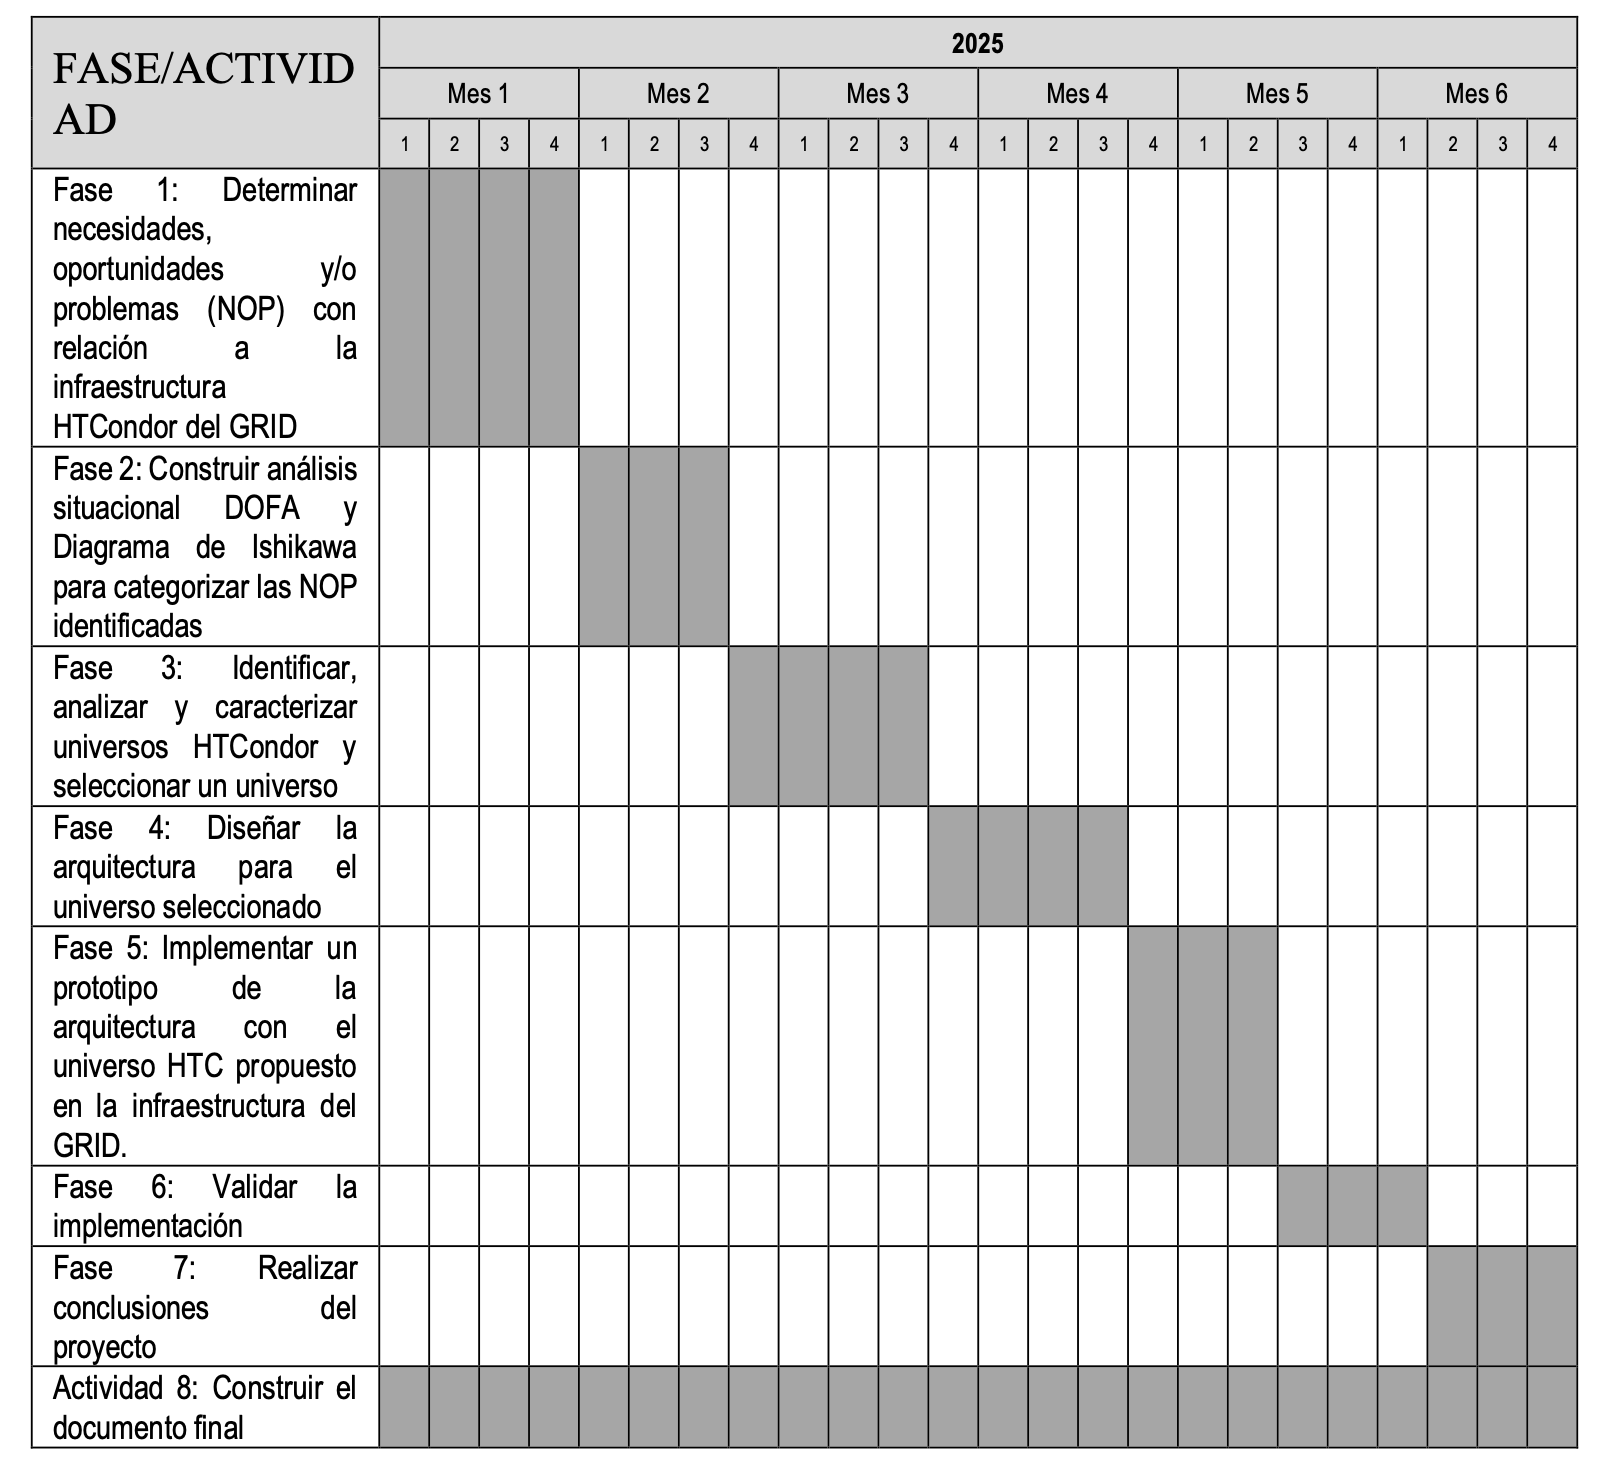
\includegraphics[scale=0.5]{tablas-images/partes/01-generalidades/cronograma.png}
	\caption{Cronograma de actividades del proyecto.}\label{fig:cronograma}
\end{figure}
